\documentclass[../../main]{subfiles}

\renewcommand\thesection{\arabic{section}}


\begin{document}

\section{Drawbacks of TinyML} \label{sec:}

\subsection{Low Fidelity Nature}

The con of a sword is that it's sharp. Just like that, TinyML's
greatest advantage is it's greatest disadvantage. It is essential
to compress the size of the model to fit with the constrains of the
host device. In this process the model could turn into a \emph{low fidelity}
one.

But in most cases this will be fine, as the low fidelity one can
still infer useful information from the surroundings. Another useful
technique to increase the performance of the overall system is to
\emph{cascade} the low fidelity one with a high fidelity one.

\subsection{Cascaded Systems}

One way to deal with low fidelity models is to cascade it with
a high fidelity model. Figure \ref{fig:cascadingMLModels} shows
such a system.

\begin{figure}
    \centering
    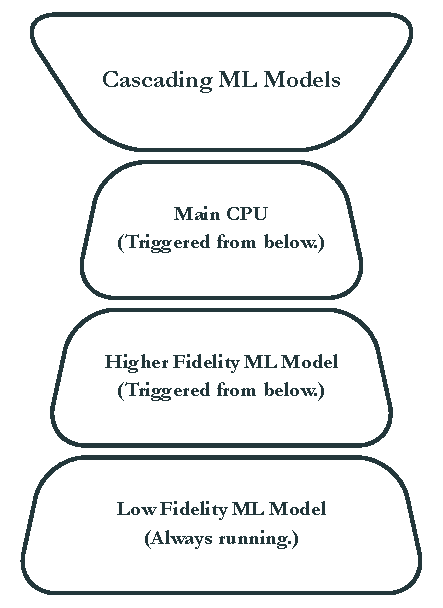
\includegraphics [
        max width = \IGXMaxWidth,
        max height = 0.3\textheight,
        \IGXDefaultOptionalArgs,
    ] {pics/cascading_ml_models.pdf}
    \captionof{figure} {Cascading different fidelity ML models.}
    \label{fig:cascadingMLModels}
\end{figure}

In this case, the low fidelity one will run continuously and consumes
the least amount of energy. Once it picks up something it can wake
up the higher fidelity one to run more inferences. If the higher fidelity
one confirms the lower fidelity one's inferences, then it can trigger
other parts of the system.

In this way, the low fidelity one can help to conserve energy, by preventing
higher fidelity one from running continuously.


\end{document}
